%%
%% 研究報告用スイッチ
%% [techrep]
%%
%% 欧文表記無しのスイッチ(etitle,eabstractは任意)
%% [noauthor]
%%

%\documentclass[submit,techrep]{ipsj}
\documentclass[submit,techrep,noauthor]{ipsj}



\usepackage[dvipdfmx]{graphicx}
% \usepackage[dvips]{graphicx}
\usepackage{latexsym}
\usepackage{url}

%%% 追加 %%%
\usepackage{amsmath}
\usepackage[hang,small,bf]{caption}
\usepackage[subrefformat=parens]{subcaption}
\captionsetup{compatibility=false}
%%% ここまで %%%

\def\Underline{\setbox0\hbox\bgroup\let\\\endUnderline}
\def\endUnderline{\vphantom{y}\egroup\smash{\underline{\box0}}\\}
\def\|{\verb|}
%

%\setcounter{巻数}{59}%vol59=2018
%\setcounter{号数}{10}
%\setcounter{page}{1}


\begin{document}


\title{注水音を用いた容器内水位推定手法}

% \etitle{How to Prepare Your Paper for IPSJ SIG Technical Report \\ (version 2018/10/29)}

\affiliate{Rits}{立命館大学大学院情報理工学研究科}
\affiliate{JST}{科学技術振興機構さきがけ}


% \paffiliate{JU}{情報処理大学\\
% Johoshori Uniersity}

\author{藤井 敦寛}{ATSUHIRO FUJII}{Rits}[atsuhiro.fujii@iis.ise.ritsumei.ac.jp]
\author{村尾 和哉}{KAZUYA MURAO}{Rits,JST}[murao@cs.ritsumei.ac.jp]

\begin{abstract}
  日常生活において容器へ液体を注ぐ場面は多数存在する.陶器の徳利やアルミ缶のような不透明かつ口が狭い容器に飲料などの液体を注ぐ場合,目視では容器内の水位を正しく把握することが困難であり,液体が溢れてしまうことがある.そのため,筆者らは目視以外の何らかの手法を用いて容器内の水位を把握したいと考えた.水位の検知には液面レベルセンサの使用が考えられるが,注がれる容器ごとにデバイスを取り付ける必要があり煩雑である.そこで本研究では,容器に液体を注ぐときに発生する注水音をセンシングして容器内の水位を推定する手法を提案する.提案手法は容器外で注水音を取得して容器内の水位を推定するため,容器ごとにデバイスを取り付ける必要がなく汎用性が高い.提案手法の有効性を確認するために行った評価実験の結果,0\%--100\%の水位を10\%刻みで推定する場合,容器に依存した推定モデルでは平均0.462,依存しない推定モデルでは平均0.308という推定精度が得られた.一方で,水位が90\%以上であるか否かを推定するモデルの場合,容器に依存せずとも平均0.744という推定精度が得られた.これは水位推定の場合は精度を改善する必要があるが,溢れ検知においては提案手法を実環境で使用できる可能性があることを示している.今後は満水になる直前に注水を停止する機能を組み込んだ蛇口取り付け型デバイスを実装していく.
\end{abstract}


%
%\begin{jkeyword}
%情報処理学会論文誌ジャーナル,\LaTeX,スタイルファイル,べからず集
%\end{jkeyword}
%
%\begin{eabstract}
%This document is a guide to prepare a draft for submitting to IPSJ
%Journal, and the final camera-ready manuscript of a paper to appear in
%IPSJ Journal, using {\LaTeX} and special style files.  Since this
%document itself is produced with the style files, it will help you to
%refer its source file which is distributed with the style files.
%\end{eabstract}
%
%\begin{ekeyword}
%IPSJ Journal, \LaTeX, style files, ``Dos and Dont's'' list
%\end{ekeyword}

\maketitle

% 1
\section{はじめに}
日常生活において容器へ液体を注ぐ場面は多数存在する.ガラスのコップのように内部の状況が視認できる容器に液体を注ぐ場合は,容器内の水位を把握できるため液体が溢れることは少ないが,陶器の徳利やアルミ缶のような不透明かつ口が狭い容器に液体を注ぐ場合,目視では容器内の水位を正しく把握することが困難であり,液体が溢れてしまうことがある.水や飲料を注ぐ場合であれば溢れても拭き取ればよいが,ペンキのような液体は拭き取ることが難しい.灯油やガソリンなどの危険性の高い液体が溢れた場合,事故に繋がる恐れがある.そのため,筆者らは目視以外の何らかの手法を用いて容器内の水位を把握する必要があると考える.水位を把握する既存研究として,Renら\cite{LiquidSense}は水位識別システムであるLiquidSenseを提案している.このシステムでは既存のホームWi-Fiネットワークを利用し,低コストのトランスデューサを容器の表面に取り付けることで,容器の共振を検知して液面レベルを識別する.そのほか,マイクロコントローラ向けに小型の液面レベルセンサが市販されている\footnote{\url{http://sfe.io/p10221}}.しかしながら,これらの手法やセンサを利用して水位を識別するには,容器ごとにデバイスを取り付ける必要がある.\par

容器を加工することなく水位を取得するには,超音波センサを設置して水面までの距離によって水量を推定する方法\cite{smart_faucet1}が考えられる.しかし,蛇口にセンサを設置する場合,容器を手に持って注水すると蛇口から容器までの距離が一定ではないため水位の推定が難しくなる.そのほか,蛇口にカメラを設置して画像認識することにより水量の推定を行う方法が考えられるが,暗所では識別精度が低下してしまう可能性がある.また,水が斜め向きに放出されるような蛇口も存在するため,口径が小さい容器へ注水する際に正しく距離を取得できない可能性がある.\par

そこで本研究では,容器に液体を注ぐときに発生する注水音をセンシングして容器内の水位を推定する手法を提案する.提案手法は容器外で注水音を取得し容器内の水位を推定するため,容器ごとにデバイスを取り付ける必要がなく汎用性が高い.音の特徴を使用した推定手法であるため,暗所でも推定精度への影響はない.また,蛇口や容器の口径の変化による影響も受けにくいと考えられる.本稿では容器に液体を注ぐときに発生する音を注水音と表現するが,容器に液体を注ぐ際に音が発生する状況であれば,注ぐ液体は水に限らず水位の推定が可能である.提案手法はマイクのみを利用するため,さまざまな環境に設置できる.溢れる直前に注水を停止するスマート蛇口としての実装や,スマートフォン用のアプリケーションとしての実装も考えられる.ガソリンの給油ノズルにはベンチュリ効果を用いた自動給油停止装置が実装されているが,バイクのような小さなガソリンタンクへの給油時には装置が動作せず,手動で溢れないように調整する必要がある.しかし,ガソリンタンクの給油口は口径が小さく目視による内容量の確認は難しい.スマートフォン用のアプリケーションとしての実装は,このような場面で有効である.給油時にスマートフォンを給油口の横で把持しておくだけでガソリンタンクの内容量を推定し,溢れる前に通知する.溢れの防止は資源の無駄使いを減らし,ひいては環境保全にも繋がると考えている.本稿ではさまざまなデバイスへの実装の前段階として,注水音を使用した水量の推定が可能であるかを調査する.\par

以降,\ref{sec:related}節で関連研究を紹介し,\ref{sec:method}節で提案手法の詳細を説明する.\ref{sec:evaluation}節で提案手法の評価を行い,\ref{sec:future_work}節で今後の計画を述べ,最後に\ref{sec:conclude}節で本研究をまとめる.

% 2
\section{関連研究}
\label{sec:related}
本節ではスマートホームの推進,音による識別,水量推定に関する研究を紹介する.

% 2.1
\subsection{スマートホームの推進}
Xuら\cite{smart_home1}はスマートフォンやタブレットのアプリケーション上で豆の温度や一酸化炭素量の監視が可能なスマートコーヒーロースタを提案している.
Hiraiら\cite{smart_home2}はさまざまな情報を同時に表示することが可能な天井を利用したディスプレイシステムを提案している.
Hossainら\cite{smart_home3}は浴槽内での人間の活動を認識することにより,安全性の向上や節水を可能にするセンサベースのスマートバスタブシステムを提案している.
そのほか,スマート冷蔵庫に関する研究\cite{smart_refrigerator1, smart_refrigerator2, smart_refrigerator3, smart_refrigerator4}も存在する.
このようにスマートホームの推進に向けてさまざまなスマートデバイスに関する研究が行われている.\par

また,Chiuら\cite{PlayfulBottle}は携帯電話を日常的に使用するマグカップに装着し,オフィスワーカが健康的な量の水を飲むように動機づけるシステムを提案している.
Tommyら\cite{SmartBottle}はAndroidスマートフォン用のアプリケーションを通じて水の消費量をリアルタイムにデータ化し,ユーザに通知する機能を持つスマートボトルを提案している.ボトルとスマートフォンはシームレスなBluetoothで接続される.
Kanerら\cite{GROW}はユーザに定期的に水を飲むことを促すことを目的にデザインされたスマートボトルのプロトタイプ``Grow''を開発している.内蔵された液面センサにより毎日の水の摂取量を記録し,ボトル表面をアンビエントディスプレイとして利用してフィードバックを与える.

Al-Yemniら\cite{smart_faucet2}は,体温に応じた水温に調整した水を吐出するスマート蛇口を提案している.Arduino Unoを使用して実装され,温度センサと冷水,温水の2つのバルブを制御することで実現した.提案されたデバイスは水温を調整する間の無駄な水の吐出の削減を可能にする.また,古い設備であっても蛇口を取り替えるだけで利用可能である.
Sawidinら\cite{smart_faucet3}は,Arduino Unoを制御システムとしたスマートホームコントロールシステムを設計している.設計されたシステムはAndroidスマートフォンから照明のon/off,家のドアやガレージの開閉のほか,水栓の開閉を操作できる.
これらはボトルや蛇口のスマートデバイス化に関する研究だが,水量の推定を目的とする研究ではない.


% 2.2
\subsection{音による識別}
Katoら\cite{sound_sensing1}は,直感的なユーザインタフェースの実現に向けて,手首部分に対するアクティブ音響センシングによる手の状態認識手法を提案している.骨伝導音のパワースペクトル密度を特徴量として,サポートベクタマシン(SVM)によって状態認識を行う.
Liら\cite{Auto++}は,ユーザのスマートフォンに内蔵されたマイクから取得された音響信号を用いて,車両の接近を検知するシステムを提案している.提案されたシステムは車両の存在を検知するだけでなく走行方向を推定したり,ユーザの周りにいる車両の台数を算出することも可能である.
Chauhanら\cite{BreathPrint}は,呼吸音に基づく生体認証システムを提案している.このシステムでは,ユーザがスマートフォンなどのマイクを鼻に近づけて呼吸ジェスチャをすることにより音声特徴を取得する.
Shihら\cite{Breeze}は,スマートフォンのマイクを使って呼吸の状態を連続的に検出し,呼吸トレーニングを行うモバイルアプリケーションを提案している.
Mujibiyaら\cite{sound_sensing2}は,身体上のある部位で生成した超音波信号を別の部位で測定することにより,身体上へのタッチやジェスチャを推測する手法を提案している.
Schneegassら\cite{SkullConduct}は,頭蓋骨の骨伝導音の個人差を利用した個人認証手法を提案している.評価実験の結果,個人識別では97.0\%の精度,個人認証では6.9\%の等誤り率(EER)を達成した.
このように,音データはさまざまな識別手法に取り入れられている.


% 2.3
\subsection{水量推定}
栗田ら\cite{GlassHarp}は,グラスハープ音響を用いたグラス内の水量推定手法を提案している.硬いプローブでグラスを弾くと音が発生する.この音はグラス内の水量により変化するため,音を使用して水量を推定することができる.マイクロフォンを装着したロボットハンドの指先でグラスをはじく評価実験を行い,提案手法が1--3\%程度の誤差で水量を推定できることを確認した.
Fanら\cite{SoQr}は,日用品の外面に取り付けてその中の内容物の量を推定するセンサSoQrを提案している.このセンサはスピーカとマイクで構成されており,容器に対して短い正弦波のプローブ音を出力する.そして,マイクで容器のインパルス応答を記録し,サポートベクタマシンを使用して容量を推定する.一般的な家庭用品19品目を用いて予測モデルの評価を10分割交差検証で行った結果,平均F値が0.96以上であることがわかった.
これらの研究は水量推定を行うものである.我々の提案する手法も水量推定が目的だが注水時に限定しており,特別な動作を行う必要や容器にデバイスを装着する必要がない.

% 3
\section{提案手法}
\label{sec:method}
本節では提案手法の詳細を述べる.

% 3.1
\subsection{概要}
提案システムの処理の流れを\figref{fig:method}に示す.手動でバルブが開放され注水が開始されるとシステムが起動し,デバイスに実装されたマイクから0.2秒間の音声データを取得する.次に特徴抽出を行い,得られた特徴量を推定モデルに投入する.最後に,推定モデルから出力された水位$W$と閾値$T_{level}$の大小比較を行い,その結果に応じてバルブを制御する.$W<=T_{level}$の間はバルブを開放したままで音声データの取得からの処理を繰り返し行う.そして,$W>T_{level}$となった段階でバルブを閉じ注水を停止してシステムを終了する.なお,手動でバルブが閉じられた場合にもシステムを終了する.

\begin{figure}[!t]
  \centering
  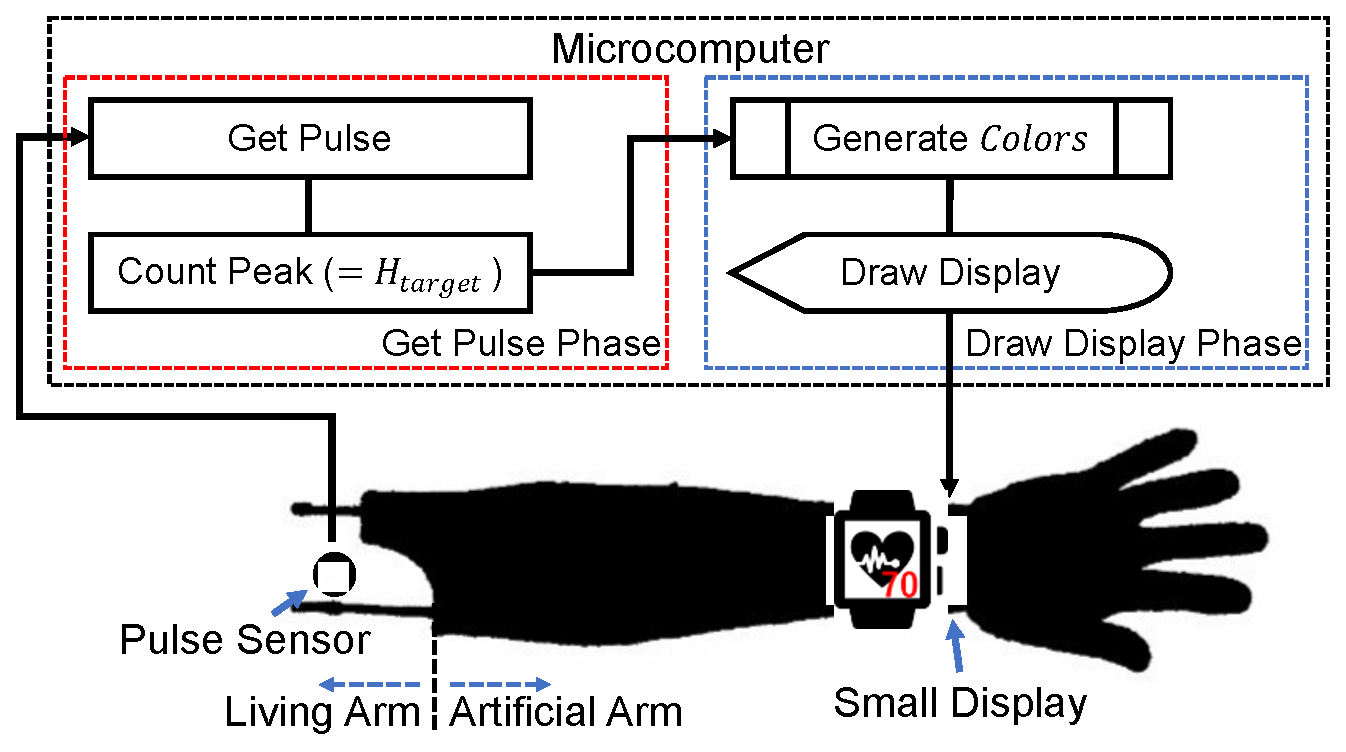
\includegraphics[width=1\linewidth]{figures/method.eps}
  \caption{提案システムの処理の流れ}
  \label{fig:method}
\end{figure}


% 3.2
\subsection{特徴抽出}
特徴量には音声認識で一般的に使用されているメル周波数ケプストラム係数(MFCC)の時間平均を用いた.MFCCの算出にはPythonの音響信号処理ライブラリであるLibROSA\footnote{\url{https://librosa.org}}の\texttt{librosa.feature.mfcc}メソッド\footnote{\url{https://librosa.org/doc/main/generated/librosa.feature.mfcc.html}}を使用した.ここで,MFCCの次元数を指定する引数$n\_mfcc$は61と設定した.算出されたMFCCからデータの直交成分を表している1次元目のデータを削除した後,時間平均を計算し1次元で長さが60の特徴量を抽出する.


% 3.3
\subsection{推定モデル}
推定モデルの構造を\figref{fig:model}に示す.モデルは3層の畳み込み層,ReLU関数,プーリング層,全結合層で構成し,全結合層から出力された値はSoftmax関数を通して生起確率に変換される.その後,Activation層で確率が最大のラベルが選択される.ただし,最大の確率が複数存在する場合はインデックスが最も小さいラベルを採用する.PyTorch\footnote{\url{https://pytorch.org}}を使用して実装し,Loss関数にはCrossEntropyLoss\footnote{\url{https://pytorch.org/docs/stable/generated/torch.nn.CrossEntropyLoss.html}},オプティマイザにはAdam\footnote{\url{https://pytorch.org/docs/stable/generated/torch.optim.Adam.html}}を使用した.Adamのパラメータ$lr$は0.0002と設定した.また,Conv1dおよびMaxPool1dで使用するカーネルサイズは3と決定した.CrossEntropyLossにはSoftmax関数が組み込まれているため,学習時には全結合層から出力された値をそのまま使用する.

\begin{figure*}[!t]
  \centering
  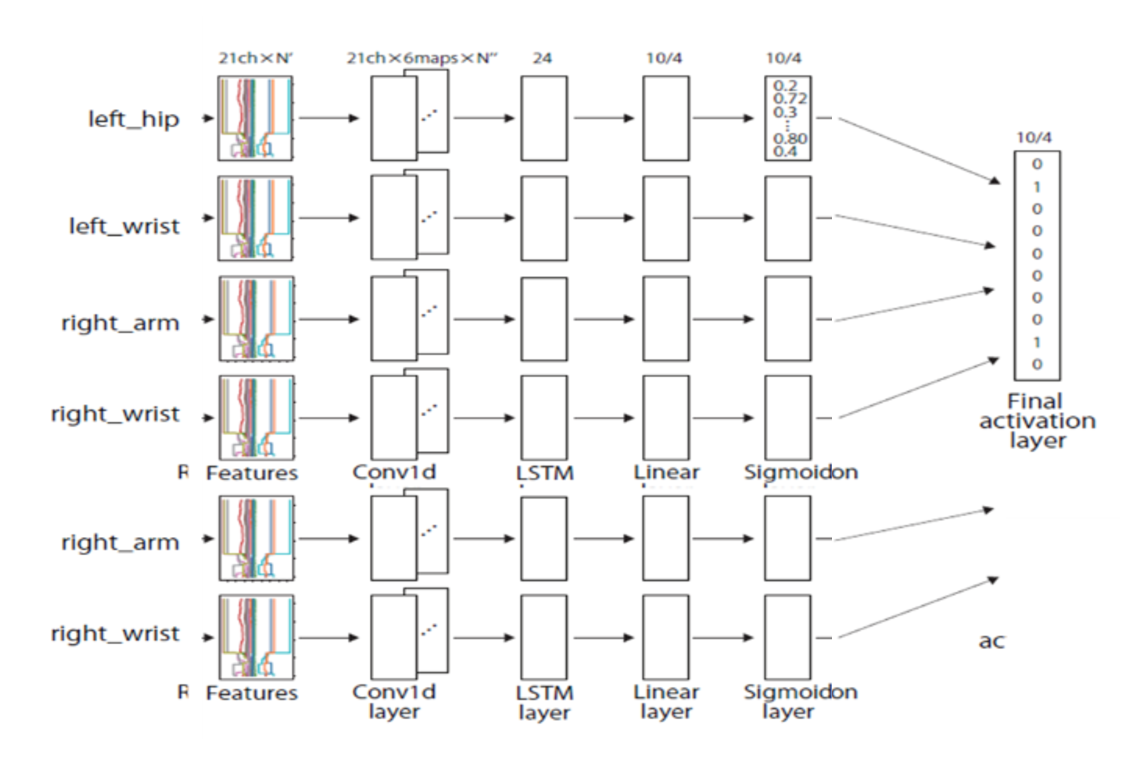
\includegraphics[width=0.8\linewidth]{figures/model.eps}
  \caption{推定モデルの構造}
  \label{fig:model}
\end{figure*}



% 4
\section{評価}
\label{sec:evaluation}
提案手法の有効性を確認するため,事前に収集した注水音データを使用して評価実験を行った.

% 4.1
\subsection{データの収集}
注水音の録音にはAndroidスマートフォン(OPPO Find X3 Pro)に標準搭載されているボイスレコーダアプリケーションを使用し,以下の流れでデータを収集した.はじめに,蛇口を一定の開度にして水を流す.次に,片方の手にスマートフォンを持ち,反対の手に容器を持つ.容器を水が入る位置まで近づけ,スマートフォンは容器に触れない程度まで近づける.容器に水が入り始めた瞬間にアプリケーション上の録音開始ボタンを押下し,水が溢れる瞬間に録音終了ボタンを押下する.この1回の録音で得られた注水音データを1サンプルとする.録音中の様子を\figref{fig:data_acquisition}に示す.蛇口の開度を一定にしたまま,サンプリング周波数96kHzで\figref{fig:bottles}に示す各容器から20サンプルずつ(合計100サンプル)のデータを収集した.容器は左から順にコーヒーのアルミ製の空き缶(Bottle A),プラスチック製の食器用洗剤の空き容器(Bottle B),プラスチック製のシャンプーボトル(Bottle C),プラスチック製の乳液の空き容器(Bottle D),陶器製の徳利(Bottle E)であり,素材や形状が異なる.

\begin{figure}[!t]
  \centering
  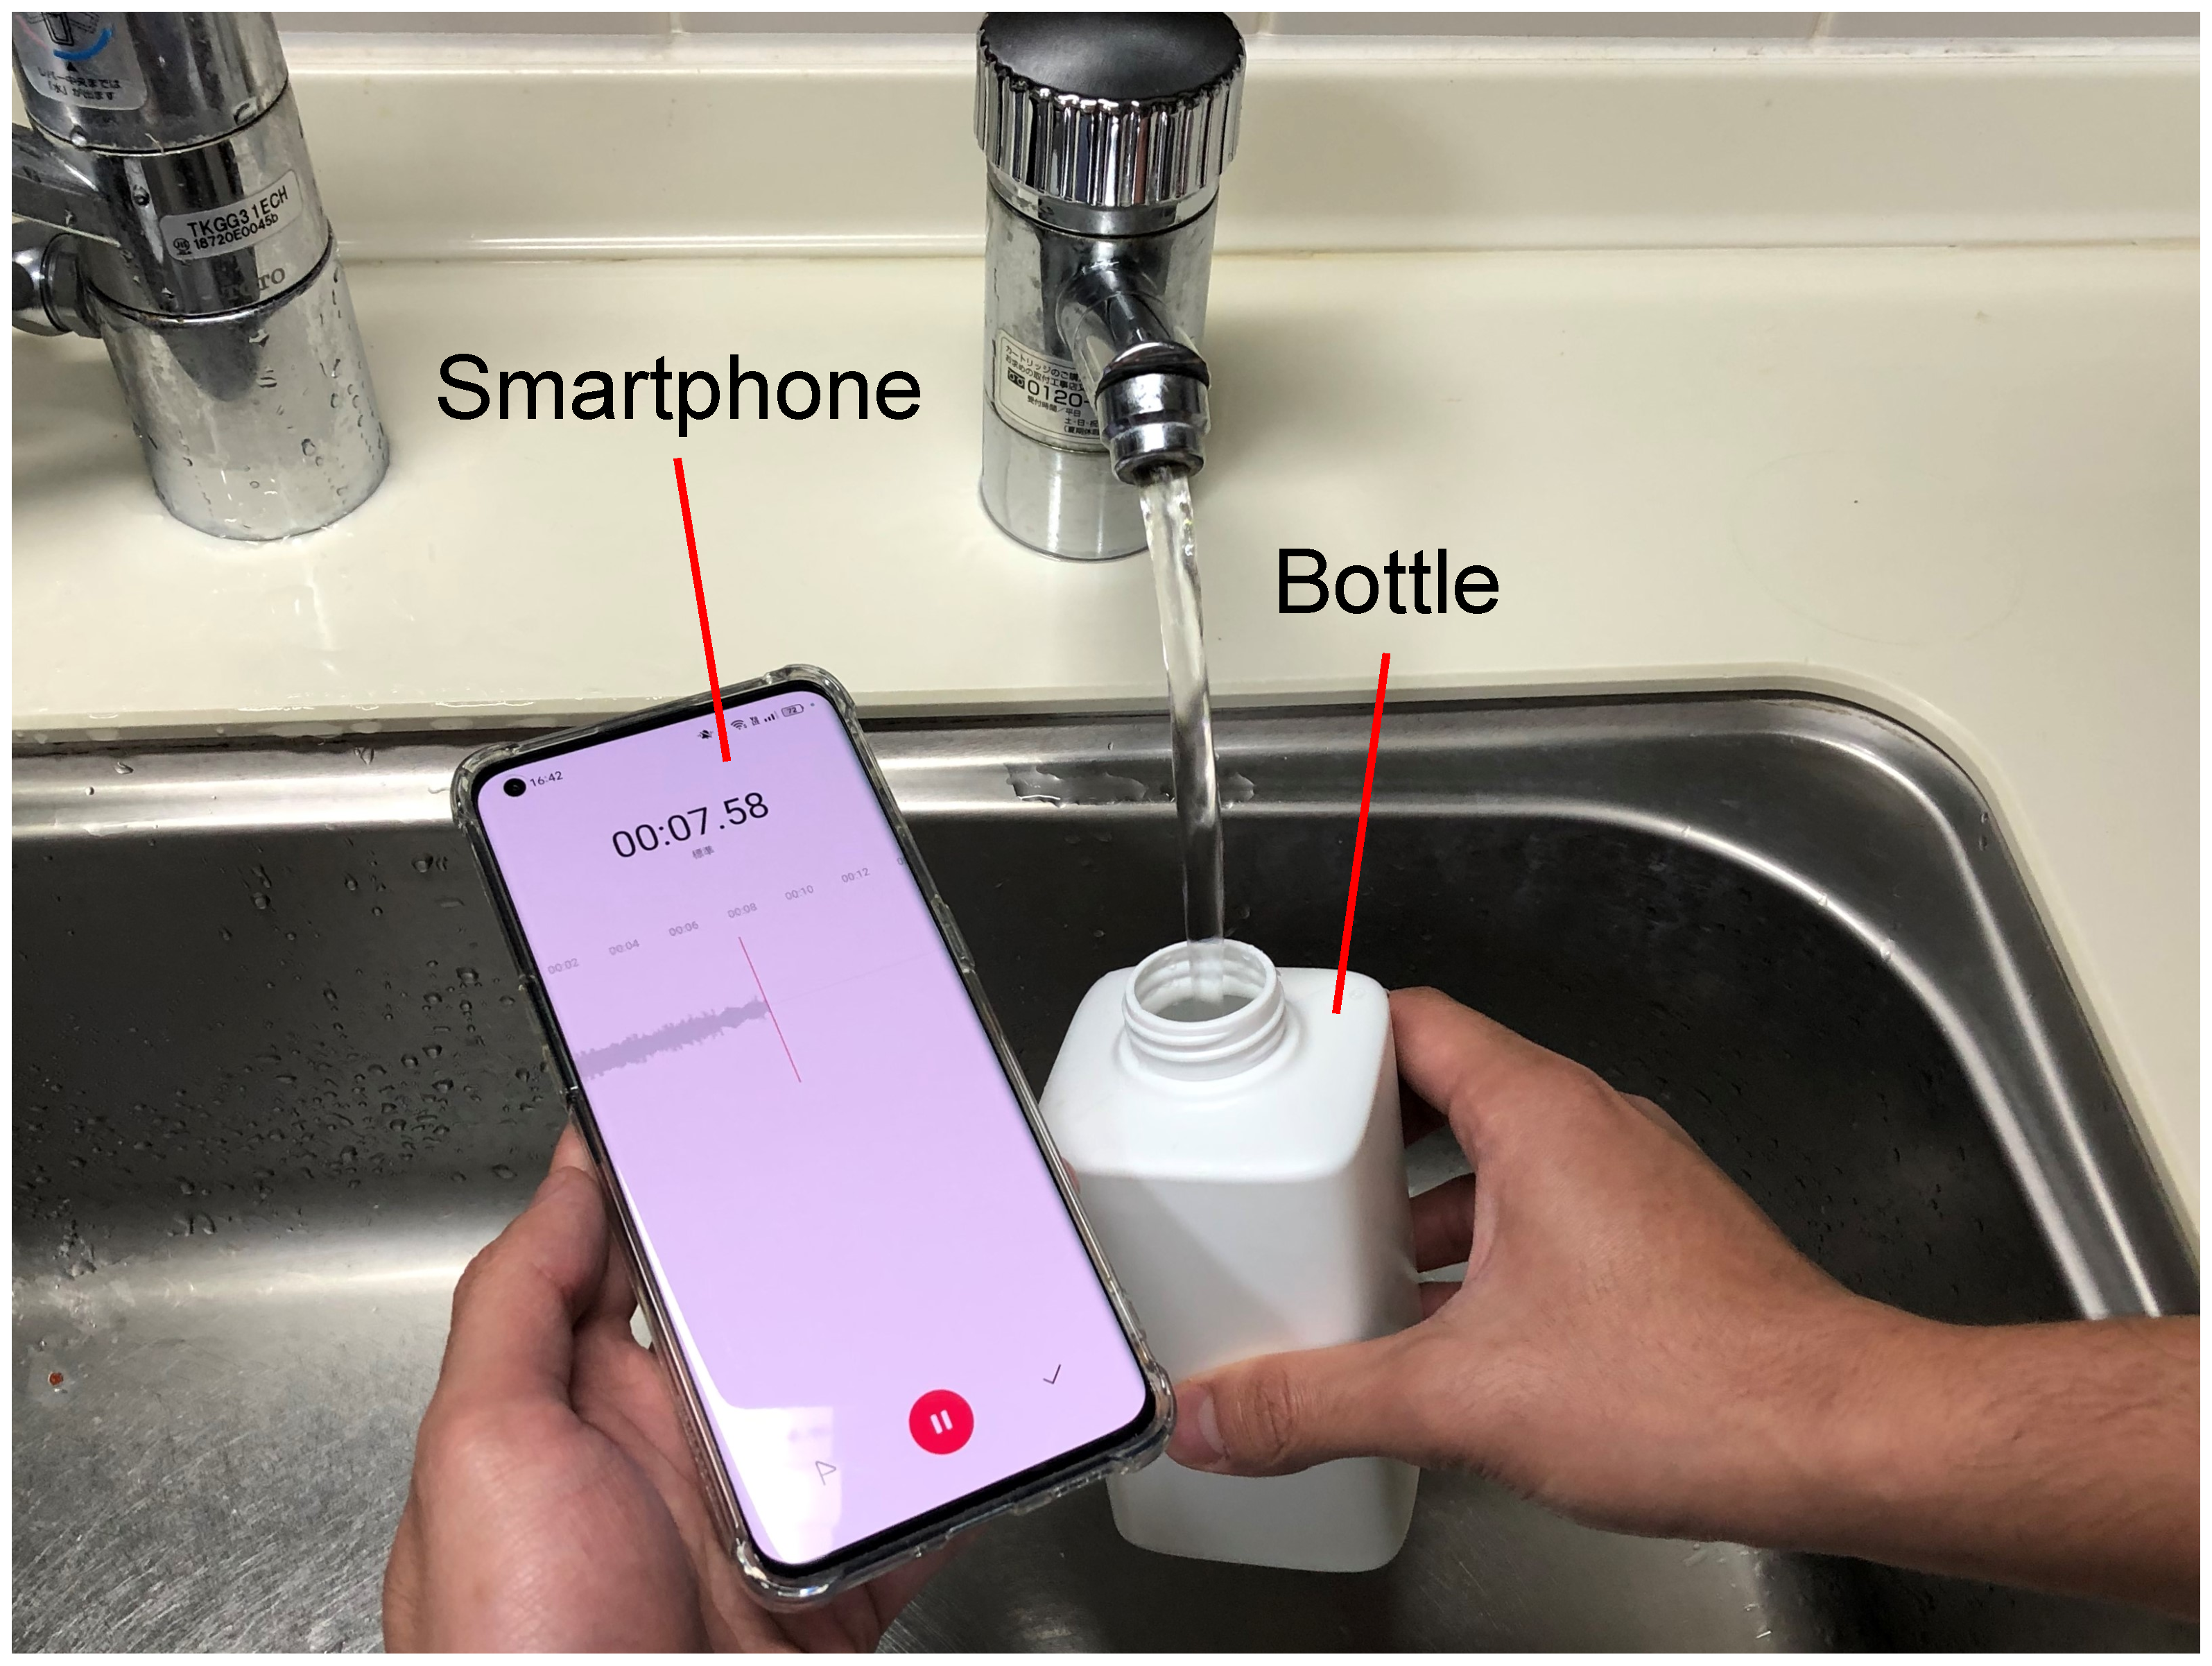
\includegraphics[width=1\linewidth]{figures/data_acquisition.eps}
  \caption{データ収集の様子}
  \label{fig:data_acquisition}
\end{figure}

\begin{figure}[!t]
  \centering
  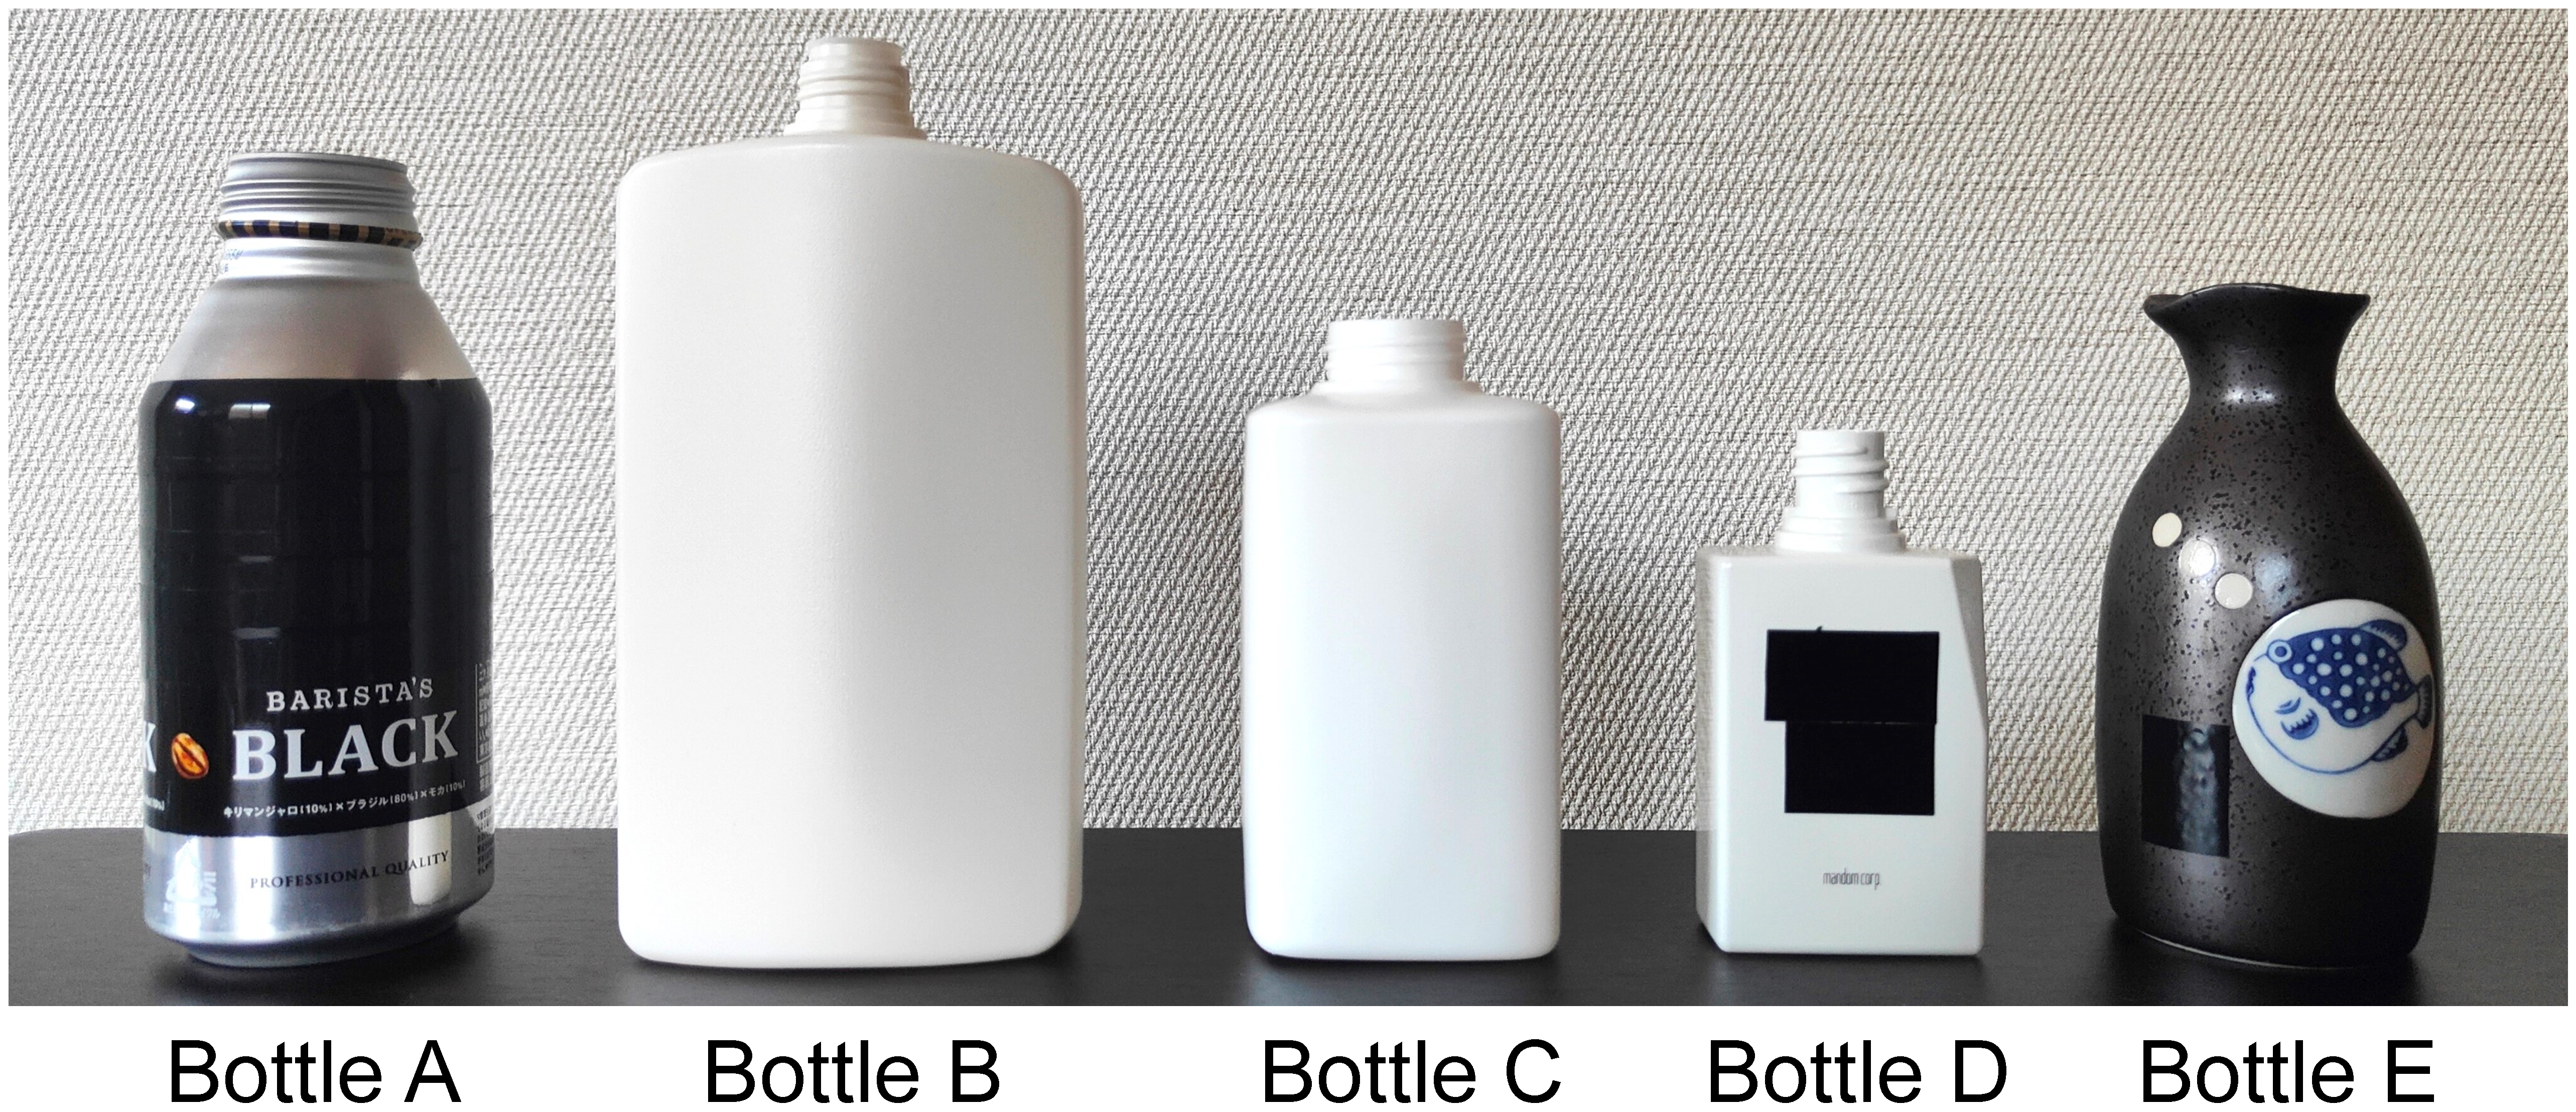
\includegraphics[width=1\linewidth]{figures/bottles.eps}
  \caption{評価に使用した容器}
  \label{fig:bottles}
\end{figure}


% 4.2
\subsection{評価環境}
収集した注水音データはあらかじめ水位のラベルを付与しておく.このとき,長さ$L$の注水音の$i$番目のデータである$x[i]$ $(i=0,\dots,L-1)$に付与される$y[i]$は次式で求めた.
\begin{equation}
  y[i]=i \times 100/(L-1)
\end{equation}
その後,ウィンドウサイズ0.2秒,ステップ幅0.02秒のスライディングウィンドウでセグメンテーションを行う.なお,ラベルはウィンドウ末尾のデータに付与されたものを使用する.\par

識別クラス数は$C=[BOTTLES\_NUM,10,2]$とし,それぞれモデルを構築した.このとき,全結合層の出力次元数を識別クラス数と同一に変更した.$C=BOTTLES\_NUM$(本稿では5)のときは注水されている容器の種類を識別する.$C=10$のときは0--100\%の範囲の水位を10\%刻みで識別する.一方で,$C=2$の場合は水が溢れるか否かに着目し,90\%以上の水位であるかどうかを識別する.識別モデルの学習フェーズにおけるバッチサイズは100,エポック数は1,000とした.1エポックの学習に使用するデータは容器と水位のデータが均等に含まれるように調整した.具体的には,$C=[BOTTLES\_NUM,10]$のときはA(0\%--10\%), A(10\%--20\%), \dots, A(90\%--100\%), B(0\%--10\%), \dots, E(80\%--90\%), E(90\%--100\%)から,$C=2$のときはA(0\%--90\%), A(90\%--100\%), B(0\%--90\%), \dots, E(0\%--90\%), E(90\%--100\%)から均等にデータが含まれるようにする.また,実環境での使用を想定して容器に依存しない推定モデルも作成した.容器非依存モデルの場合にはテストに使用する容器のデータはすべて学習に使用しない.


% 4.3
\subsection{結果と考察}
本節では収集した注水音データを使用して水位の識別精度を調査する.

% 4.3.1
\subsubsection{容器推定モデル}
容器の種類を識別するモデルについて,全容器の合計100サンプルのデータのうち99サンプルを学習に使用し,学習に使用していない残り1サンプルのデータから50セグメントを抽出して精度をテストする.100サンプルのすべてがテストデータとなるようにLOSO(leave-one-session-out)アルゴリズムで精度を算出し,容器ごとの平均値を\tabref{tab:result_5}に示す.Averageは表に示した精度の平均値を表す.結果はすべて小数点第四位を四捨五入している.また,すべての予測結果を合計した混同行列を\figref{fig:confusion_matrix_5}に,学習フェーズにおける容器ごとの平均のLossの推移を\figref{fig:loss}に示す.混同行列は縦方向に入力された実際のラベル,横方向に出力された予測ラベルの個数を表す.\par

結果より平均で0.642という精度が得られた.5クラス分類でチャンスレベルの精度となる0.2と比較すると高い精度であることから,注水音を用いて容器の種類を識別することは可能であると考えられる.その一方で,容器ごとの結果ではBottle Cの識別精度が0.559と最も悪い.ここで混同行列のBottle Cに識別されたデータを確認すると,実際にはBottle Aのものであるデータを多く誤識別してしまっていることがわかる.これはBottle AとBottle Cの注水音が類似していた可能性があることを示しており,形状や口径の大きさが似ていたことが原因であると考えられる.

\begin{table}[!t]
  \small
  \centering
  \caption{容器推定精度($C=BOTTLES\_NUM$)}
  \begin{tabular}{c|c} \hline\hline
    容器 & 精度 \\ \hline
    A & 0.587 \\
    B & 0.643 \\
    C & 0.559 \\
    D & 0.666 \\
    E & 0.755 \\ \hline
    Average & 0.642 \\ \hline
  \end{tabular}
  \label{tab:result_5}
\end{table}

\begin{figure}[!t]
  \centering
  \includegraphics[width=1\linewidth]{figures/confusion_matrix_5.eps}
  \caption{容器推定における混同行列}
  \label{fig:confusion_matrix_5}
\end{figure}

\begin{figure}[!t]
  \centering
  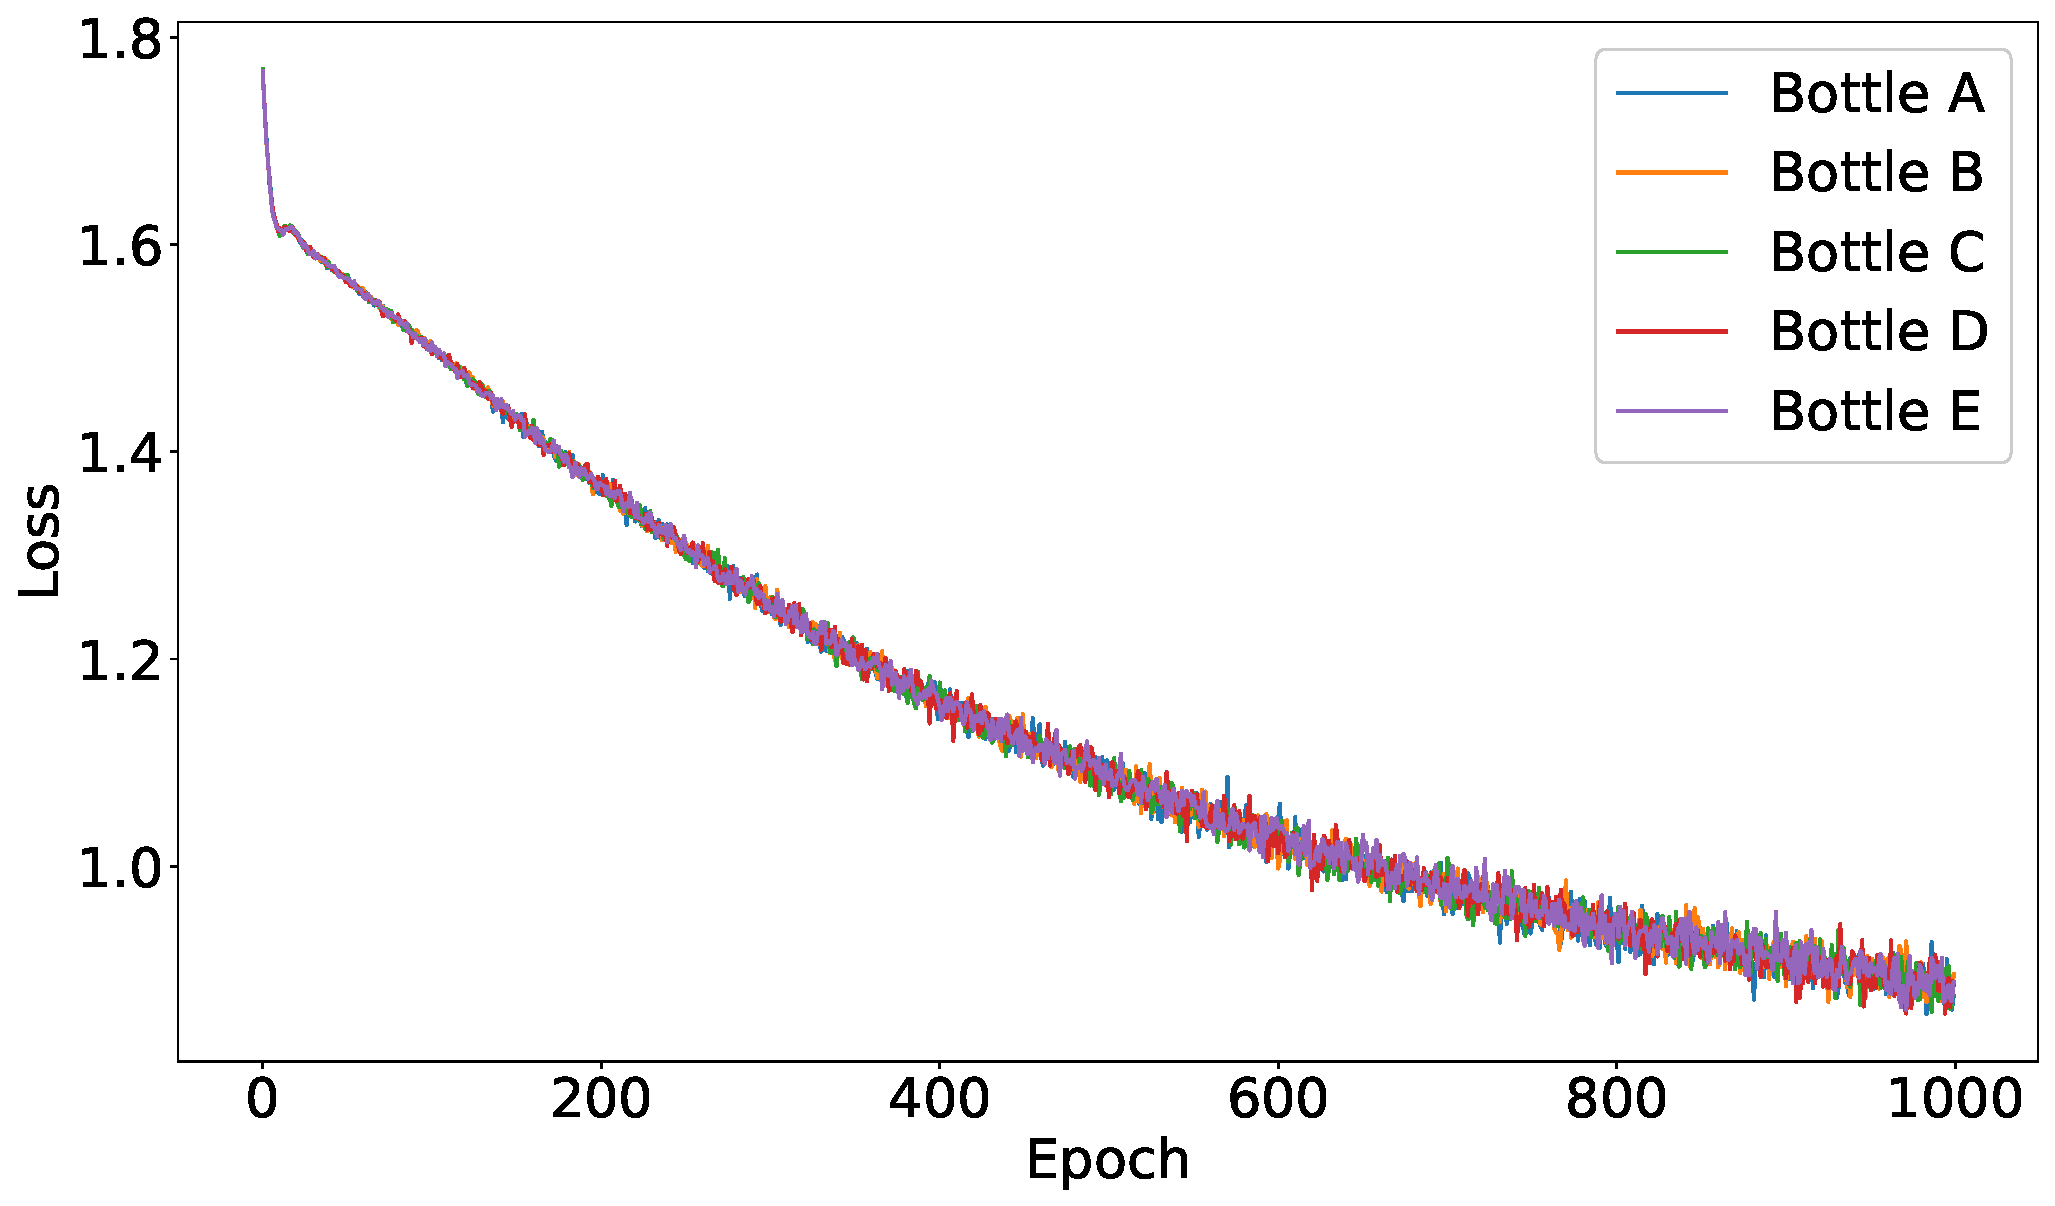
\includegraphics[width=1\linewidth]{figures/loss_5.eps}
  \caption{Lossの推移}
  \label{fig:loss}
\end{figure}

% 4.3.2
\subsubsection{水量推定モデル}
0--100\%の範囲の水位を10\%刻みで識別するモデルについて,全容器の合計100サンプルのデータのうち99サンプルを学習に使用し,学習に使用していない残り1サンプルのデータから50セグメントを抽出して容器に依存した場合の精度をテストする.100サンプルのすべてがテストデータとなるようにLOSOアルゴリズムで精度を算出し,その平均値を\tabref{tab:result_10_dependent}に,すべての予測結果を合計した混同行列を\figref{fig:confusion_matrix_10_dependent}に示す.テストデータは10クラスすべてが均一に出現するように抽出した.\par

また,4個の容器の合計80サンプルを学習に使用し,学習に使用していない残り1個の容器の20サンプルのデータから500セグメントを抽出して容器に依存しない場合の精度をテストする.5個の容器のすべてがテストデータとなるようにLOBO(leave-one-bottle-out)アルゴリズムで精度を算出し,その平均値を\tabref{tab:result_10_independent}に,すべての予測結果を合計した混同行列を\figref{fig:confusion_matrix_10_independent}に示す.テストデータは10クラスすべてが均一に出現するように抽出した.\par

結果より容器依存モデルでは平均で0.462,非依存モデルでは平均で0.308という精度が得られた.容器ごとの結果では,容器依存,非依存のどちらの場合においてもBottle Bの精度が最も悪かった.これはBottle Bの容積が最も大きかったため1サンプルから抽出されるセグメントが多くなってしまい,同じエポック数でも他の容器に比べて特徴の学習が進んでいなかった可能性がある.しかしながら,10クラス分類でチャンスレベルの精度となる0.1と比較すると高い精度であることがわかる.このことから,注水音を用いて水位を推定することは可能であると考えられる一方で,実環境での使用を考慮すると精度を改善する必要がある.混同行列を確認すると特に容器依存モデルにおいては水位が近いラベルとの誤推定が多く見られることから,推定する水位を10\%刻みから拡大するとさらに精度が向上する可能性がある.また,容器依存モデルは容器非依存モデルよりも推定精度が約0.15高いことから,似た形状の容器ごとに推定モデルを構築しておき,水位を推定する前に使用するモデルを切り替えるなどの機構を組み込むことにより大幅に精度が向上する可能性がある.

\begin{table}[!t]
  \small
  \centering
  \caption{水量推定精度($C=10$)}
  \begin{minipage}[t]{0.45\linewidth}
    \centering
    \subcaption{容器依存モデル}
    \begin{tabular}{c|c} \hline\hline
    容器 & 精度 \\ \hline
    A & 0.553 \\
    B & 0.333 \\
    C & 0.479 \\
    D & 0.424 \\
    E & 0.519 \\ \hline
    Average & 0.462 \\ \hline
    \end{tabular}
    \label{tab:result_10_dependent}
  \end{minipage}
  \begin{minipage}[t]{0.45\linewidth}
    \centering
    \subcaption{容器非依存モデル}
    \begin{tabular}{c|c} \hline\hline
    容器 & 精度 \\ \hline
    A & 0.436 \\
    B & 0.198 \\
    C & 0.374 \\
    D & 0.290 \\
    E & 0.244 \\ \hline
    Average & 0.308 \\ \hline
    \end{tabular}
    \label{tab:result_10_independent}
  \end{minipage}
  \label{tab:result_10}
\end{table}

\begin{figure*}[!t]
  \centering
  \begin{minipage}[t]{0.32\linewidth}
    \centering
    \includegraphics[width=0.9\linewidth]{figures/confusion_matrix_10_dependent_coffee.eps}
    \subcaption{Bottle A}
  \end{minipage}
  \begin{minipage}[t]{0.32\linewidth}
    \centering
    \includegraphics[width=0.9\linewidth]{figures/confusion_matrix_10_dependent_dishwashing.eps}
    \subcaption{Bottle B}
  \end{minipage}
  \begin{minipage}[t]{0.32\linewidth}
    \centering
    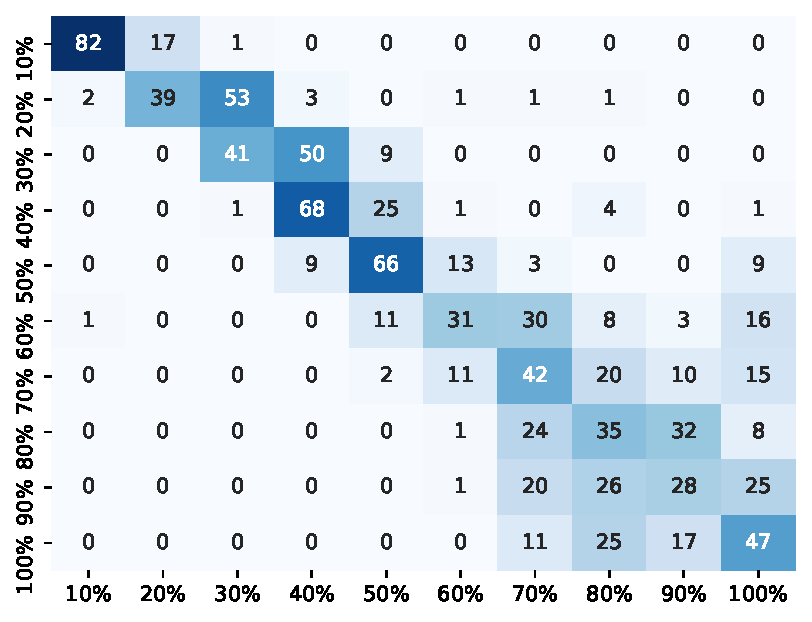
\includegraphics[width=0.9\linewidth]{figures/confusion_matrix_10_dependent_shampoo.eps}
    \subcaption{Bottle C}
  \end{minipage}
  \begin{minipage}[t]{0.32\linewidth}
    \centering
    \includegraphics[width=0.9\linewidth]{figures/confusion_matrix_10_dependent_skinmilk.eps}
    \subcaption{Bottle D}
  \end{minipage}
  \begin{minipage}[t]{0.32\linewidth}
    \centering
    \includegraphics[width=0.9\linewidth]{figures/confusion_matrix_10_dependent_tokkuri.eps}
    \subcaption{Bottle E}
  \end{minipage}
  \caption{水量推定における混同行列(容器依存モデル)}
  \label{fig:confusion_matrix_10_dependent}
\end{figure*}

\begin{figure*}[!t]
  \centering
  \begin{minipage}[t]{0.32\linewidth}
    \centering
    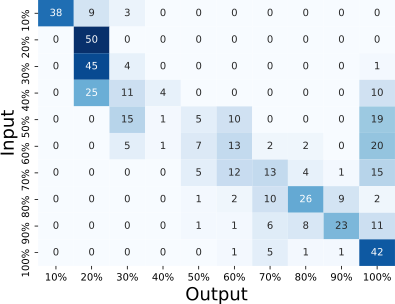
\includegraphics[width=0.9\linewidth]{figures/confusion_matrix_10_independent_coffee.eps}
    \subcaption{Bottle A}
  \end{minipage}
  \begin{minipage}[t]{0.32\linewidth}
    \centering
    \includegraphics[width=0.9\linewidth]{figures/confusion_matrix_10_independent_dishwashing.eps}
    \subcaption{Bottle B}
  \end{minipage}
  \begin{minipage}[t]{0.32\linewidth}
    \centering
    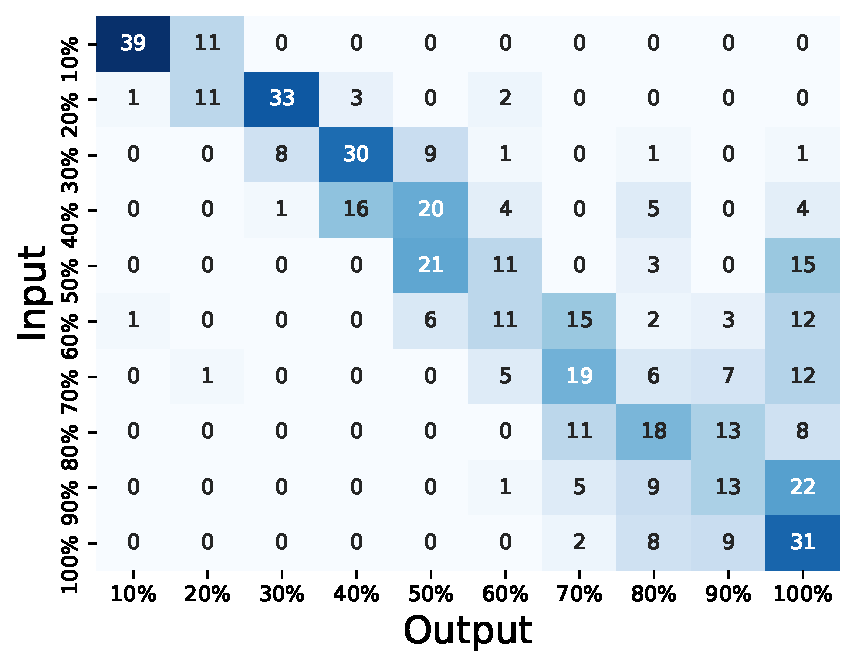
\includegraphics[width=0.9\linewidth]{figures/confusion_matrix_10_independent_shampoo.eps}
    \subcaption{Bottle C}
  \end{minipage}
  \begin{minipage}[t]{0.32\linewidth}
    \centering
    \includegraphics[width=0.9\linewidth]{figures/confusion_matrix_10_independent_skinmilk.eps}
    \subcaption{Bottle D}
  \end{minipage}
  \begin{minipage}[t]{0.32\linewidth}
    \centering
    \includegraphics[width=0.9\linewidth]{figures/confusion_matrix_10_independent_tokkuri.eps}
    \subcaption{Bottle E}
  \end{minipage}
  \caption{水量推定における混同行列(容器非依存モデル)}
  \label{fig:confusion_matrix_10_independent}
\end{figure*}

% 4.3.3
\subsubsection{溢れ検知モデル}
水が溢れるか否かに着目し,90\%以上の水位であるかどうかを識別するモデルについて,全容器の合計100サンプルのデータのうち99サンプルを学習に使用し,学習に使用していない残り1サンプルのデータから30セグメントを抽出して容器に依存した場合の精度をテストする.100サンプルのすべてがテストデータとなるようにLOSOアルゴリズムで精度を算出し,その平均値を\tabref{tab:result_2_dependent}に示す.テストデータは推定する0\%--90\%,90\%--100\%の2クラスが均一に出現するように抽出した.\par

また,4個の容器の合計80サンプルを学習に使用し,学習に使用していない残り1個の容器の20サンプルのデータから500セグメントを抽出して容器に依存しない場合の精度をテストする.5個の容器のすべてがテストデータとなるようにLOBOアルゴリズムで精度を算出し,その平均値を\tabref{tab:result_2_independent}に示す.テストデータは推定する0\%--90\%,90\%--100\%の2クラスが均一に出現するように抽出した.\par

結果より,容器依存モデルでは平均で0.83,非依存モデルでは平均で0.744という精度が得られたことから,容器に依存せずとも溢れる直前に検知できることが明らかになった.高い精度で検知できていることから,蛇口取り付け型デバイスへの実装が可能であると考えられる.また,0\%--90\%,90\%--100\%という推定クラスの幅を0\%--80\%,80\%--100\%に広げることにより,さらなる精度の向上が期待できる.

\begin{table}[!t]
  \small
  \centering
  \caption{溢れ検知精度($C=2$)}
  \begin{minipage}[t]{0.45\linewidth}
    \centering
    \subcaption{容器依存モデル}
    \begin{tabular}{c|c} \hline\hline
    容器 & 精度 \\ \hline
    A & 0.852 \\
    B & 0.755 \\
    C & 0.782 \\
    D & 0.878 \\
    E & 0.882 \\ \hline
    Average & 0.830 \\ \hline
    \end{tabular}
    \label{tab:result_2_dependent}
  \end{minipage}
  \begin{minipage}[t]{0.45\linewidth}
    \centering
    \subcaption{容器非依存モデル}
    \begin{tabular}{c|c} \hline\hline
    容器 & 精度 \\ \hline
    A & 0.760 \\
    B & 0.668 \\
    C & 0.770 \\
    D & 0.770 \\
    E & 0.750 \\ \hline
    Average & 0.744 \\ \hline
    \end{tabular}
    \label{tab:result_2_independent}
  \end{minipage}
  \label{tab:result_2}
\end{table}



% 5
\section{今後}
\label{sec:future_work}
評価実験の結果,溢れ検知モデルでは容器への依存がなくとも高い精度が得られることがわかった.しかしながら,水量推定モデルでは容器依存の場合においても平均0.462という精度にとどまった.今後は,水量推定モデルの精度向上のため,容器ごとに水量推定モデルを構築しておき,容器識別モデルから得られた結果に応じて水量推定モデルを切り替える手法や,連続した5つのウィンドウの識別結果から多数決を行い,その結果を採用する手法を検討している.また,提案手法を組み込んだ蛇口取り付け型デバイスを実装し,その効果を評価していく.



% 6
\section{まとめ}
\label{sec:conclude}
本研究では,内部状況が把握しづらい容器でも水位を正しく把握することができるように,蛇口に取り付けたデバイスで注水音を取得して容器内の水位を推定する手法を提案した.識別モデルを実装し,5個の容器を使用して識別精度の評価実験を行った.その結果,容器識別モデルは平均0.642,水位推定モデルは容器依存の場合では平均0.462,非依存の場合では平均0.308,溢れ検知モデルは容器依存の場合では平均0.83,非依存の場合では平均0.744という精度だった.この結果は水位推定の場合は精度を改善する必要があるが,溢れ検知においては容器に依存せずとも識別が可能であり実環境で使用できる可能性があることを示している.今後は推定精度の向上のためのモデルの改善のほか,注水時において満水になる直前に注水を停止する機能を組み込んだ蛇口取り付け型デバイスを実装していく予定である.





\bibliographystyle{ipsjunsrt}
\bibliography{references}

\end{document}
